\subsection{Target}

The CLAS12 target components are imported from the engineering model. The STEP files are converted to tessellated STL files and imported
in the GEMC simulation \cite{targetCorrection, targetStudy}. An example of the tessellation is shown in \F{targetScatteringChamber}.

Key elements of the STL import include the Torlon tube to the target cell,
the target aluminum windows, the Kapton walls, and the scattering chamber (see \F{targetDesign}).
An overview of the target in Geant4 and the engineering model is shown in \F{targetOverview}.

\begin{figure}
	\centering
	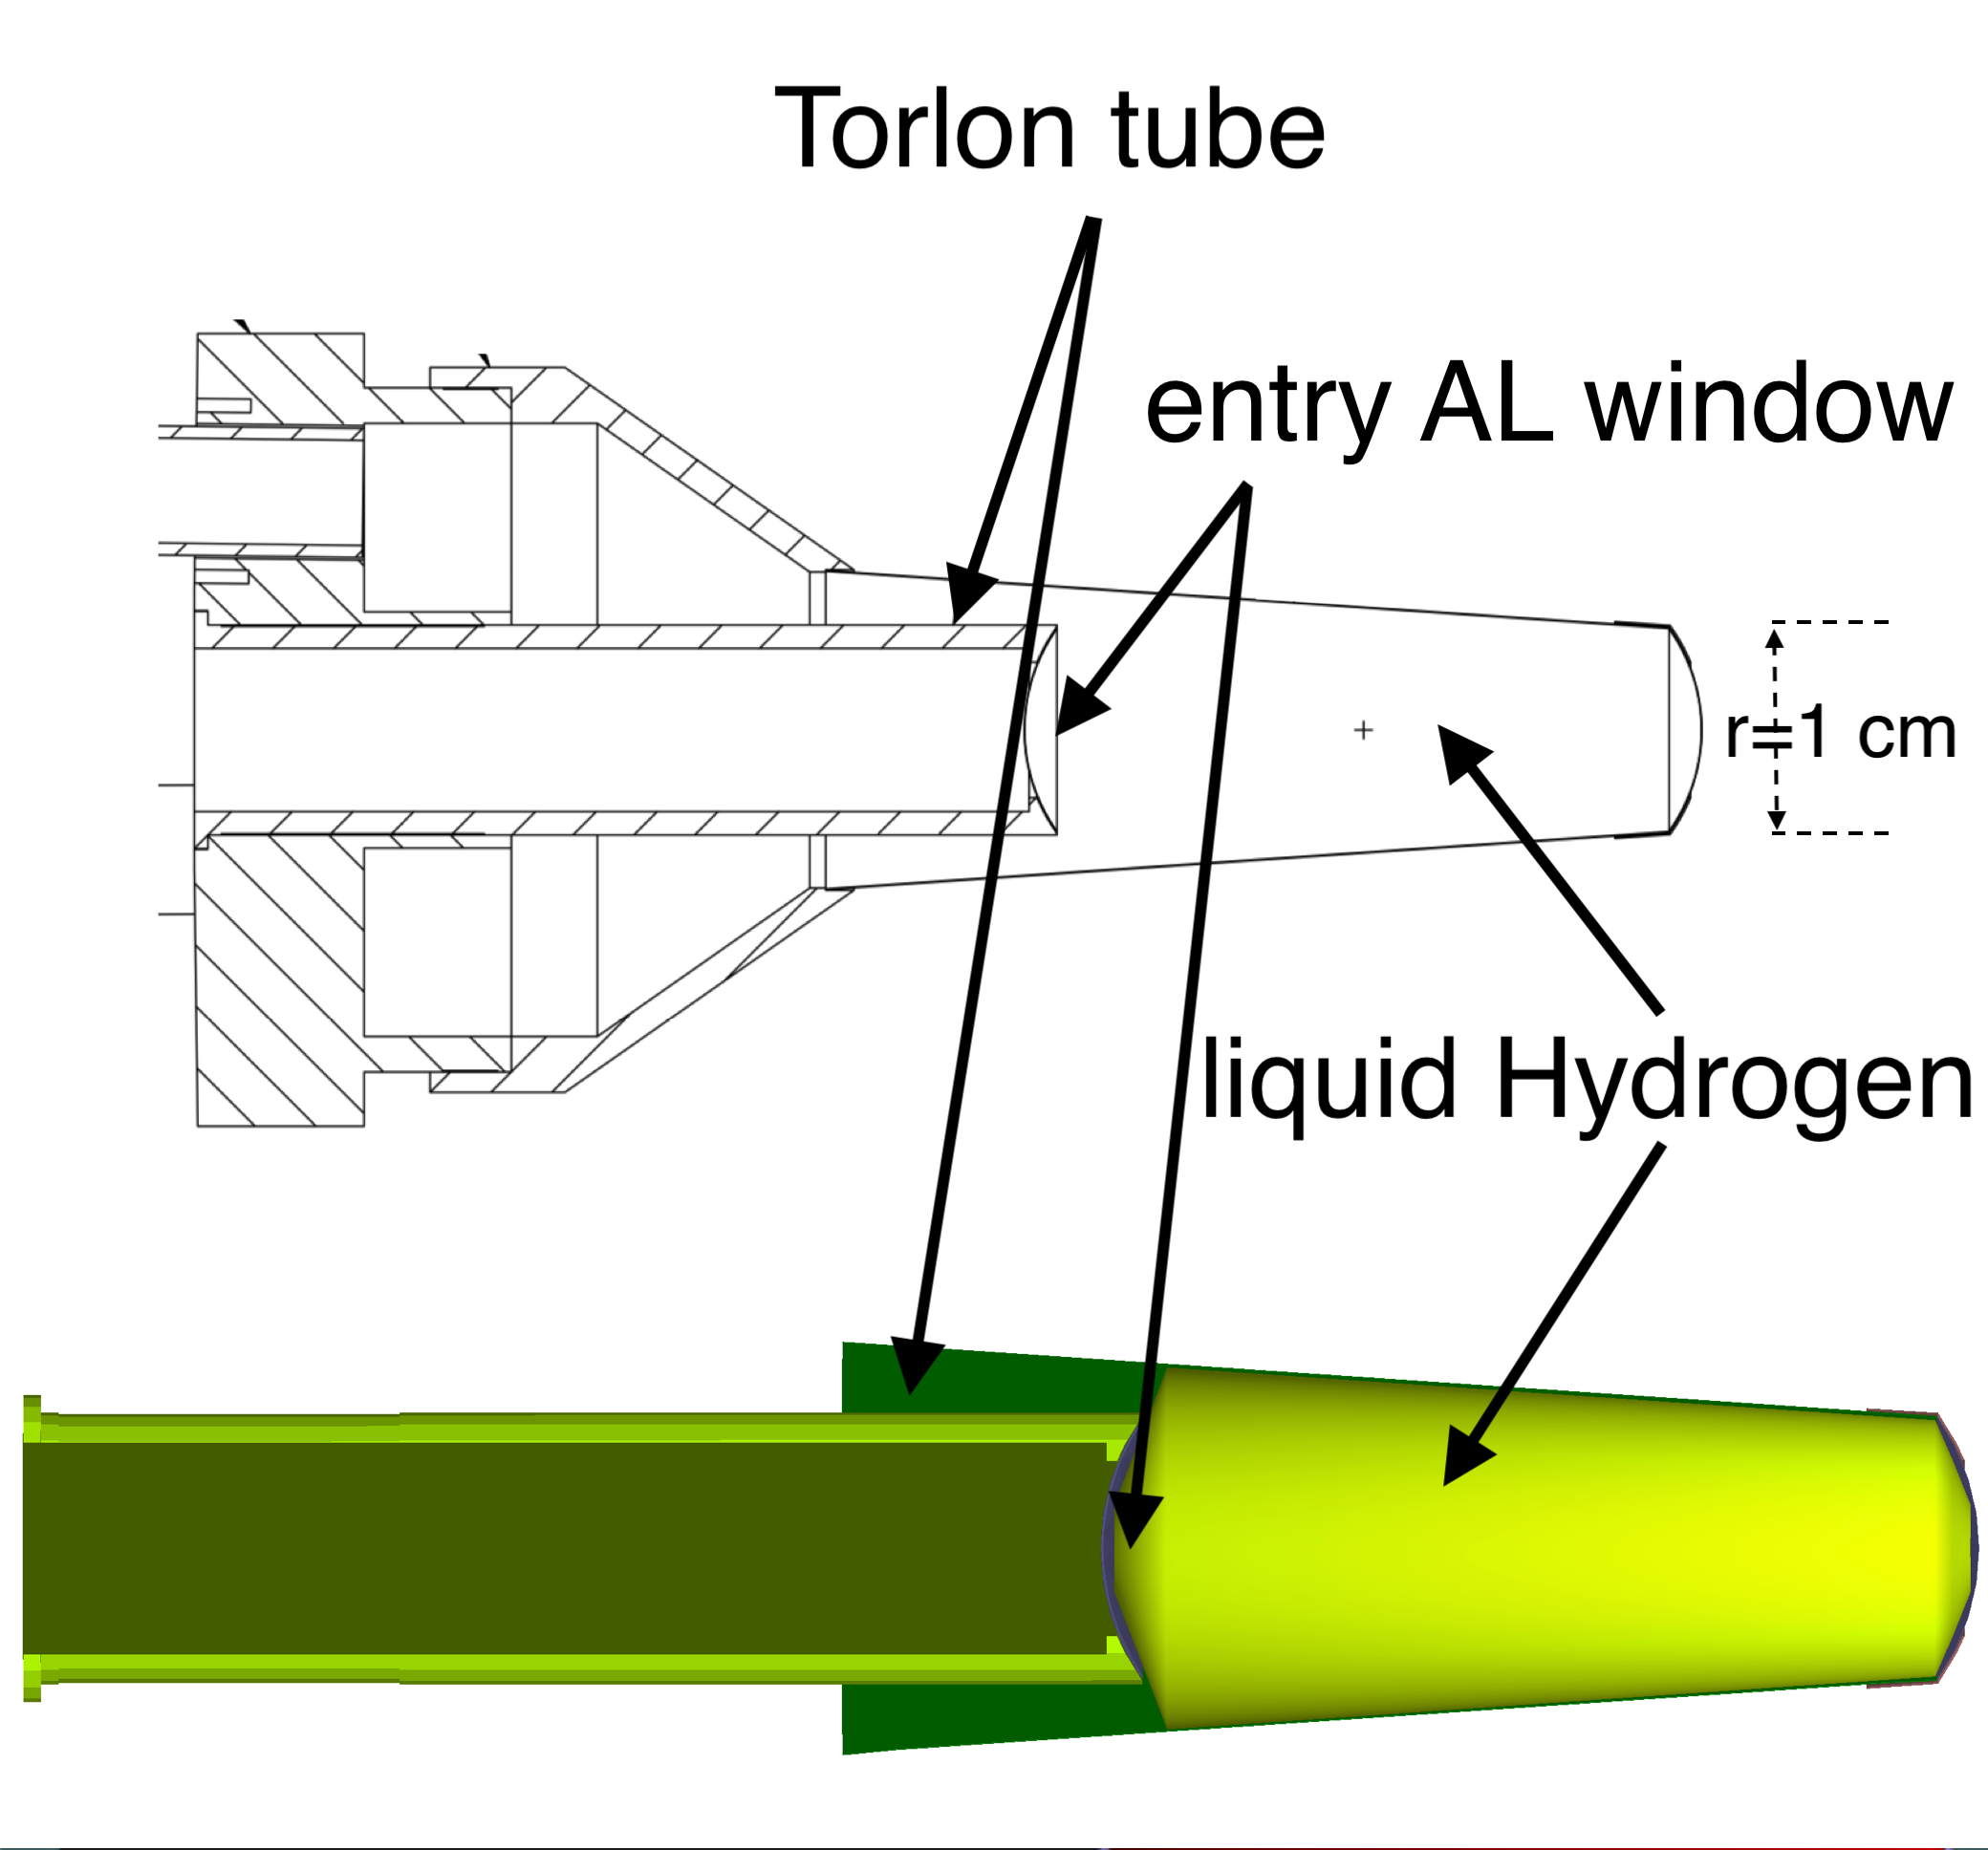
\includegraphics[width=0.99\columnwidth,keepaspectratio]{img/targetDesign.png}
	\caption{(Color Online) The CLAS12 target. Top: the engineering model of the liquid-hydrogen cell design: the outer radius is
             tapered down from 1.5 cm at $z$=-2.5 cm to 1.0 cm at $z$ = 2.5 cm.
             Bottom: The GEMC implementation of the CLAS12 target from the CAD drawings. From left to right (beam direction):
             the Torlon tube, the upstream aluminum window, the target cell, the Kapton cap, and the
			 downstream aluminum window. Notice that only the volumes that may affect the measurements are imported.}
	\label{fig:targetDesign}
\end{figure}


\begin{figure}
	\centering
	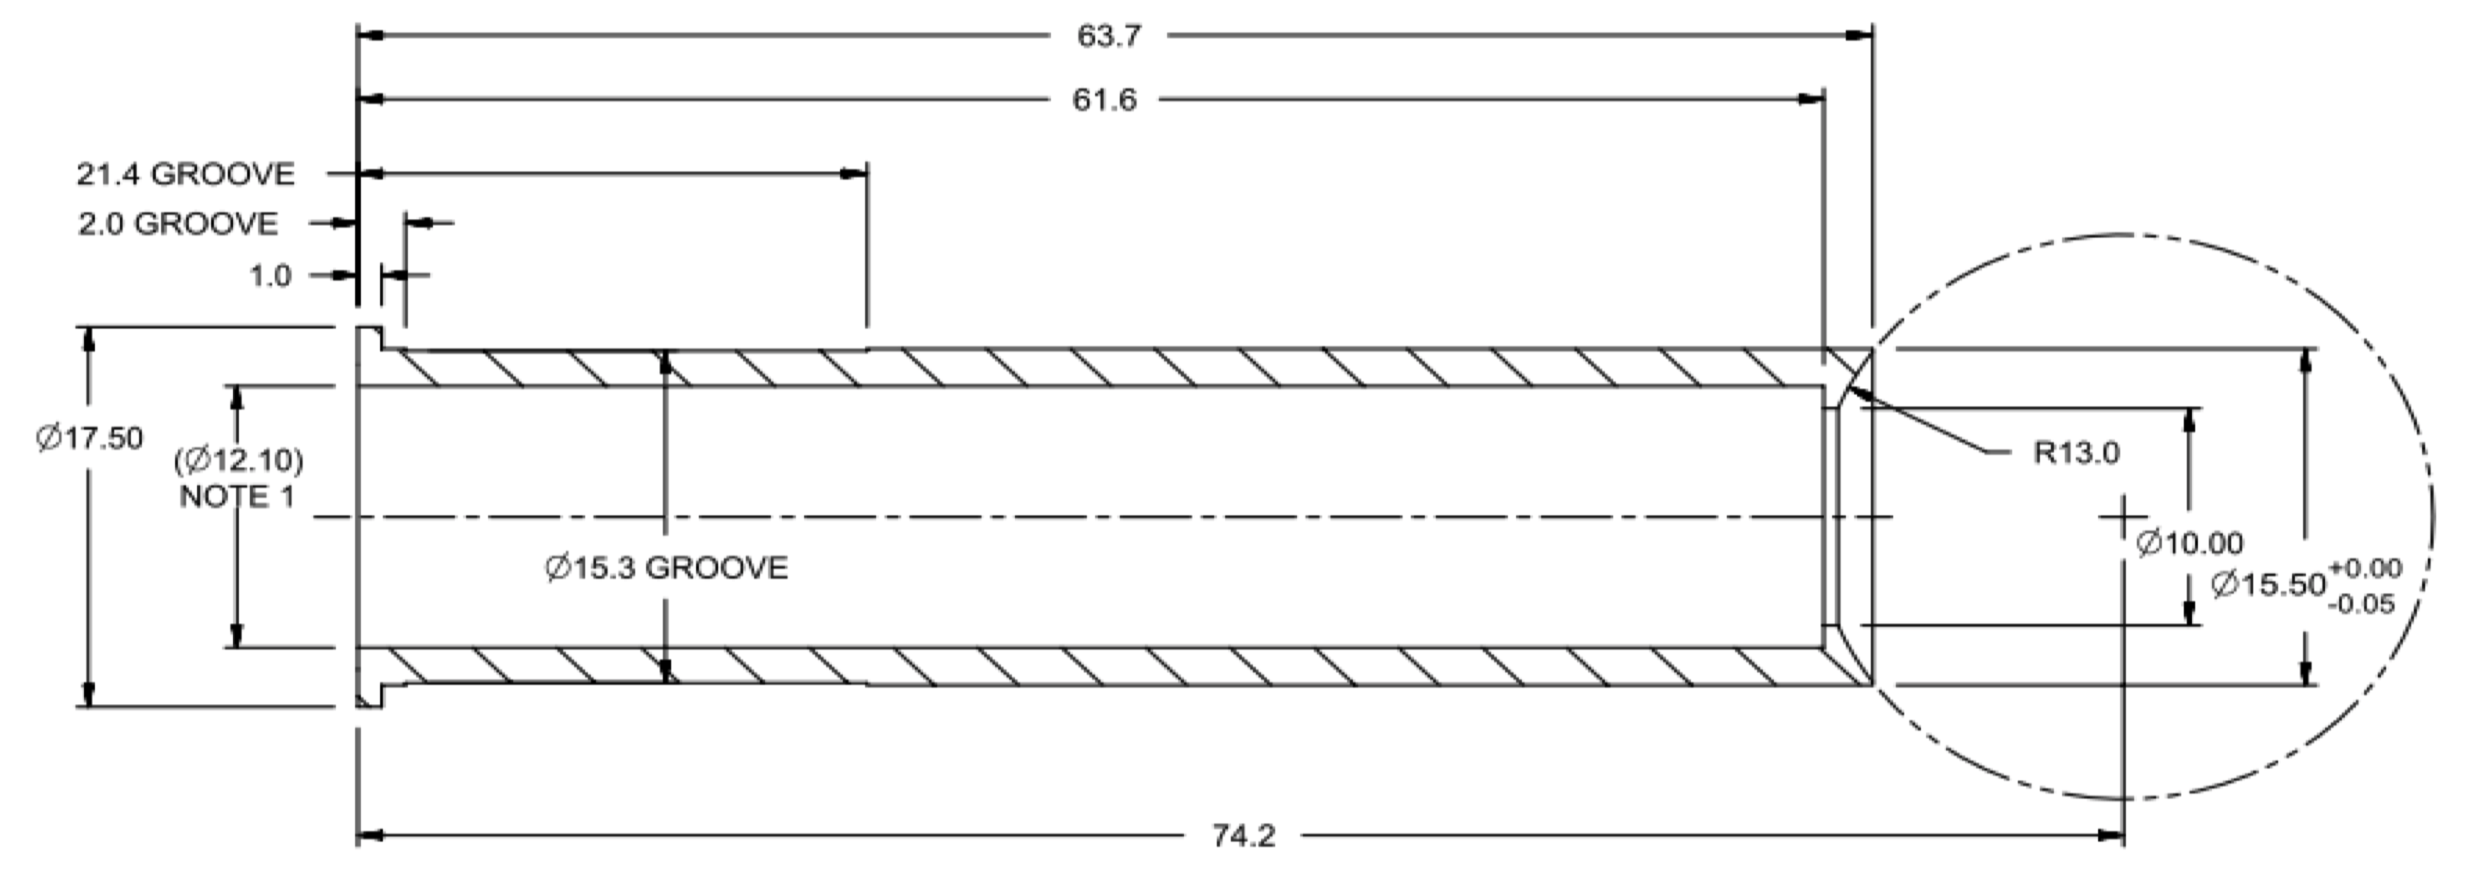
\includegraphics[width=0.99\columnwidth,keepaspectratio]{img/targetOverview2.png}
	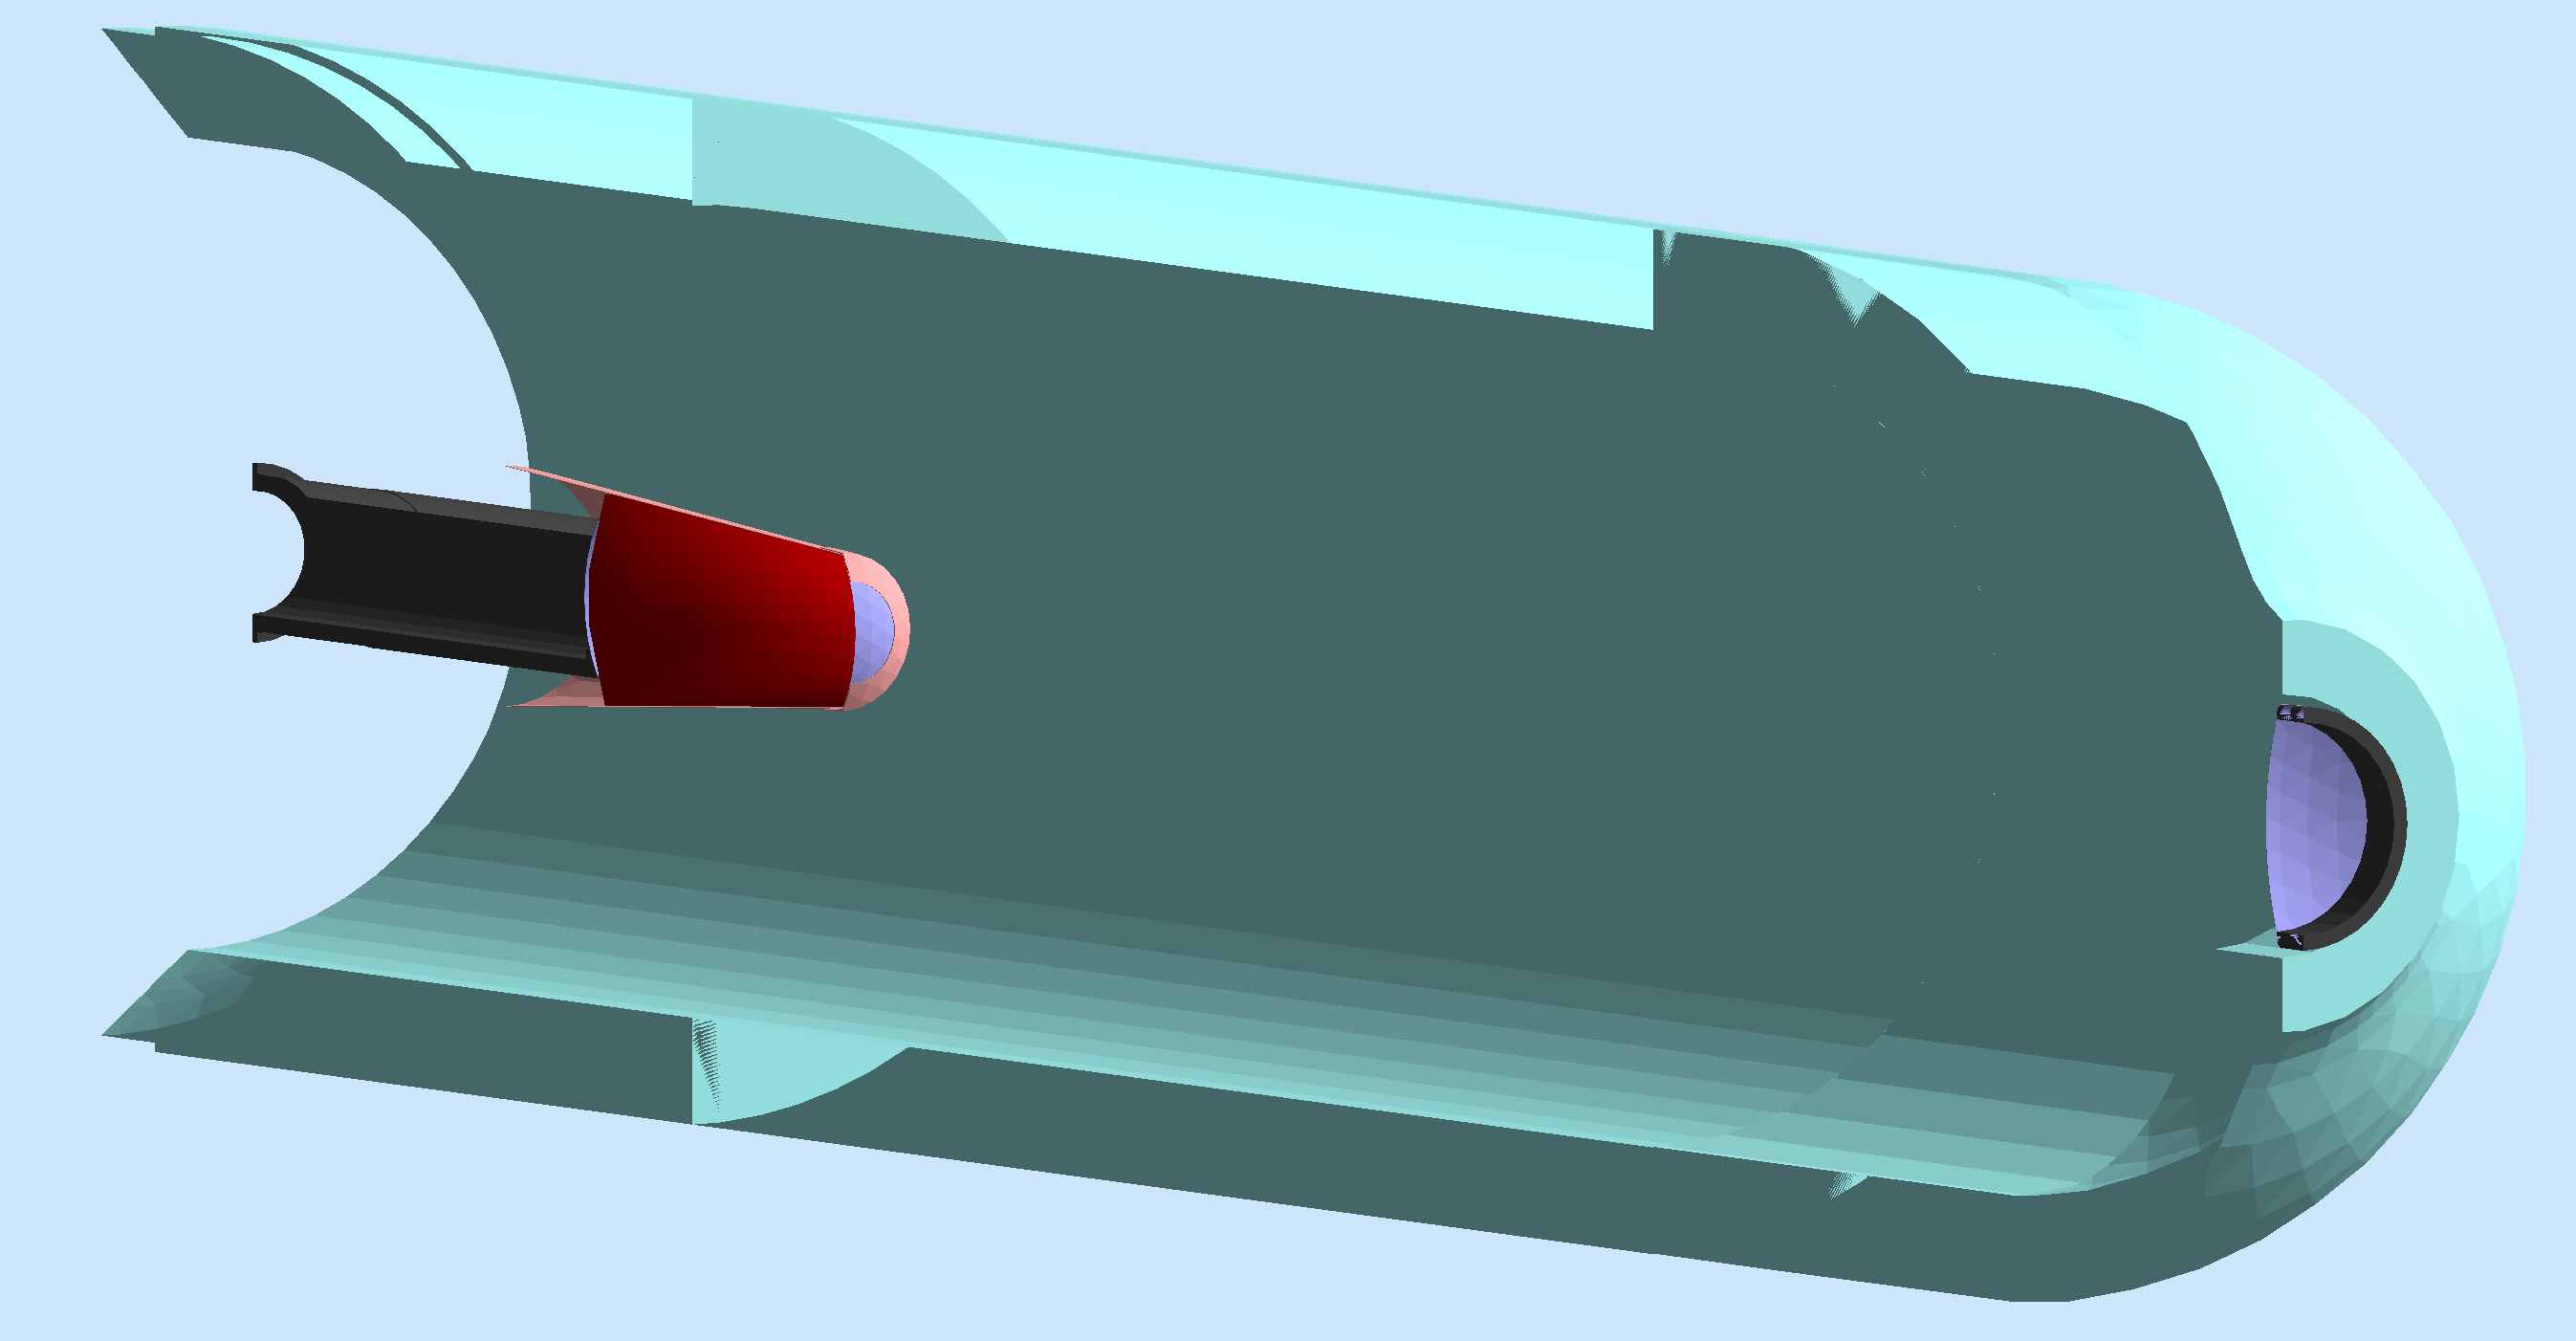
\includegraphics[width=0.99\columnwidth,keepaspectratio]{img/targetOverview1.png}
	\caption{(Color Online) Top: the CLAS12 target system engineering model. This includes the support, cooling system, scattering chamber, and
			 liquid-hydrogen cell. The circle highlights the part imported in the simulation.
			 Bottom: overview of the target implementation in GEMC includes the foam scattering chamber (light color), the
			 cell (also shown in \F{targetDesign}) and, on the right, the downstream Kapton cap containing the 50 $\mu$m aluminum window. }
	\label{fig:targetOverview}
\end{figure}

%The Github location of the GEMC perl API scripts and the STL files is \url{https://github.com/gemc/detectors/tree/master/clas12/targets}.





